\documentclass[11pt]{article}
\usepackage[a4paper, margin=1in]{geometry}
\usepackage{hyperref}
\usepackage{amsmath} 
\usepackage{multicol}
\usepackage{float} 
\usepackage{graphicx}
\usepackage{caption}
\setlength{\belowcaptionskip}{0pt}
\usepackage{xepersian}
\settextfont{XB Zar}
\setlatintextfont{Times New Roman}

\title{الگوریتم ژنتیک هدایت شده توسط جستجوی درختی مونت کارلو برای بهینه‌سازی وزن‌های شبکه عصبی}
\author{Akshay Hebbar\\
	دپارتمان مهندسی و علوم کامپیوتر\\
	Syracuse University, New York\\
	\texttt{ahebbar@syr.edu}}

\date{}

\begin{document}
	\maketitle
	
	\begin{abstract}
		در اين مقاله، امکان استفاده از یک استراتژی جستجو در الگوریتم‌های ژنتیک برای بررسی کل ساختار درخت ژنتیک را بررسی می‌کنیم. چندین روش به انجام جستجوهای درختی کمک می‌کنند؛ اما الگوریتم‌های ساده‌تری مانند جستجوی عرضی، جستجوی عمقی، و تکنیک‌های تکراری محاسبات زیادی را نیاز دارند و اغلب منجر به زمان اجرای طولانی می‌شوند. تکنیک‌های رقابتی معمولاً مکانیزم ترجیحی در هنگام انجام جستجوی احتمالاتی هستند و نتایج بهینه را سریع‌تر به دست می‌آورند. مسئله‌ای که در این مقاله قصد داریم حل کنیم، بهینه‌سازی شبکه‌های عصبی با استفاده از الگوریتم‌های ژنتیک است. الگوریتم‌های ژنتیک (GA) درختی از حالت‌های ممکن را تشکیل می‌دهند و مکانیزمی برای پاداش‌دهی از طریق تابع برازندگی فراهم می‌کنند. جستجوی درختی مونت کارلو (MCTS) به عنوان یک استراتژی موثر جستجوی درختی در حالت‌ها و پاداش‌ها ثابت شده است؛ بنابراین، ما این رویکردها را ترکیب خواهیم کرد تا به صورت بهینه به جستجوی بهترین نتیجه‌ای که با الگوریتم‌های ژنتیک تولید می‌شود، بپردازیم.
	\end{abstract}
	
	\noindent\textbf{کلیدواژه‌ها:} الگوریتم‌های ژنتیک، درخت جستجوی مونت کارلو، بهینه‌سازی ، یادگیری تقویتی، شبکه عصبی
	
	\begin{multicols}{2}
		
		\section{مقدمه}
		الگوریتم‌های ژنتیکی به یک زیرشاخه از الگوریتم‌های تکاملی تعلق دارند که یک روش برای بهینه‌سازی بر اساس اصول انتخاب ژنتیکی فراهم می‌کنند. این الگوریتم‌ها در یادگیری ماشین و توسعه پژوهش، علاوه بر سیستم‌های بهینه‌سازی ابزار جستجو، کاربرد دارند. رویکرد استفاده شده در الگوریتم‌های ژنتیکی مشابه مفاهیم بیولوژیکی تولید کروموزوم است که شامل عملگرهایی مانند انتخاب، تقاطع، جهش، و بازترکیب می‌باشد. GA یک رویکرد مبتنی بر جمعیت است که هدف آن ارائه راه‌حل به نسل‌های متوالی است. فرایند تکامل با استفاده از GA شامل شروع با یک جمعیت تصادفی و تکامل آن با استفاده از عملگرهای تقاطع و جهش برای تولید فرزندان است. سپس بهترین راه‌حل فیلتر شده و فرایند ژنتیکی تکرار می‌شود تا هدف به دست آید. می‌توان مشاهده کرد که در فرایند الگوریتم‌های ژنتیکی، یک درخت از راه‌حل‌های ممکن تولید می‌شود و بهترین راه‌حل برای تکرارهای بعدی انتخاب می‌شود که فضای جستجو و منابع محاسباتی را محدود می‌کند. الگوریتم‌های ژنتیکی برای دامنه‌های مختلفی از مسائل مانند درختان تصمیم‌گیری، تقسیم‌بندی، طبقه‌بندی و غیره استفاده می‌شوند. با این حال، در این مقاله، تمرکز ما بر کاربرد GA در بهینه‌سازی وزن‌های شبکه عصبی خواهد بود.
		\begin{figure}[H]
			\centering
			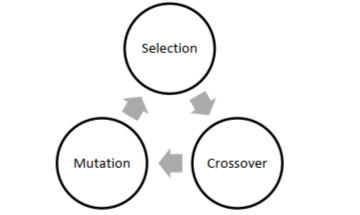
\includegraphics[width=0.4\textwidth,keepaspectratio]{1.png}
			\caption{الگوریتم ژنتیکی ساده}
			\label{fig:fig1}
		\end{figure}
		روش جستجوی درخت مونت کارلو در سال ۲۰۰۶ به عنوان یک کاربرد برای جستجوی درخت بازی توسعه یافت. این جستجوی درخت بر اساس اصول پاداش تجمعی محاسبه شده از گره‌های فرزند کار می‌کند و از مقادیر Q و N برای تعادل بین رویکردهای اکتشاف و گسترش استفاده می‌کند. رویکرد اکتشاف تعداد گره‌های بازدید شده را در نظر می‌گیرد و از یک رویکرد کمی برای کشف گره‌های فرزند که بازدید نشده‌اند استفاده می‌کند. رویکرد گسترش یک استراتژی کیفی را برای کشف گره‌های فرزند با مقدار Q که نشان‌دهنده مجموع تجمعی پاداش‌ها است دنبال می‌کند.
		\begin{figure}[H]
			\centering
			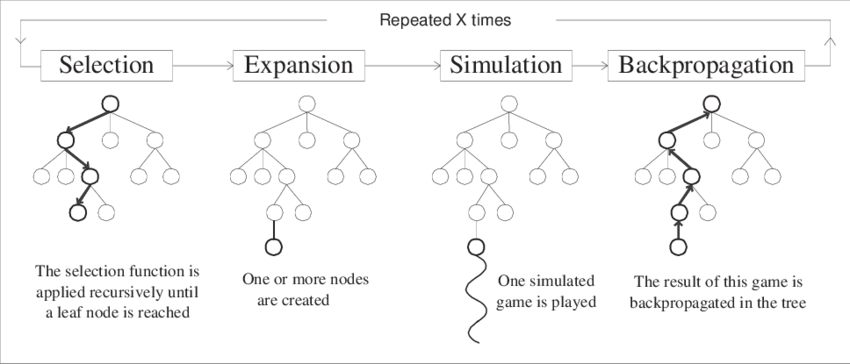
\includegraphics[width=0.49\textwidth,keepaspectratio]{2.png}
			\caption{نمای کلی از جستجوی درخت مونت کارلو}
			\label{fig:fig2}
		\end{figure}
		
		یک سیاست کافی برای MCTS - بر اساس تحقیقات قبلی - یافت شده است که UCT (درختان اعتماد به نفس بالا) می‌باشد. UCT یک حد بالای اعتماد به نفس برای جستجوی درخت فراهم می‌کند. این سیاست به جستجو کمک می‌کند تا تعادل بین اکتشاف و بهره‌برداری را حفظ کرده و فضای جستجو را بهینه هدایت کند. با توجه به اینکه MCTS یک استراتژی جستجوی درختی مقابله‌ای است، ممکن است بتوانیم آن را به کل چشم‌انداز درخت GA اعمال کنیم تا راه‌حل‌های بهینه را پیدا کنیم، به جای اینکه تنها بر اساس تناسب اکتشاف کنیم. بنابراین، در این تحقیق رویکرد جدید MCTS-GA برای بهینه‌سازی شبکه عصبی را مورد بحث قرار می‌دهیم.
		\section{توضیحات مسئله و داده‌ها}
		\subsection{الگوریتم ژنتیک‏ برای وزن‌های شبکه عصبی}
		برای بهینه‌سازی وزن‌های شبکه عصبی باید مورد توجه قرار گیرد، تایید اعتبار گره‌های فرزند تولید شده در این فرایند است. عملگرهای تقاطع و جهش اعمال شده بر این وزن‌ها ممکن است منجر به یک راه‌حل زیر بهینه در نسل‌های پایین‌تر شوند، اما این‌ها ممکن است در نسل‌های بعدی به راه‌حل‌های بهتری تبدیل شوند. به طور معکوس، یک راه‌حل که در نسل‌های اولیه بالاترین تناسب را داشته است، ممکن است در نسل‌های بعدی به یک نتیجه زیر بهینه منجر شود به دلیل ماهیت عملگرهای ژنتیکی مورد استفاده. بنابراین، تنها راه برای شناسایی بهترین راه‌حل کلی این است که کل درخت را گسترش دهیم و تناسب هر گره فرزند را محاسبه کنیم تا یک راه‌حل ارزشمند پیدا شود. با این حال، این راه‌حل محاسبات سنگینی دارد و جستجوی جامع درخت حتی در موارد درختان کوچکتر به ندرت بهینه است. تعداد گره‌ها برای یک درخت داده شده که فضای جستجو را تشکیل می‌دهد با فرمول زیر محاسبه می‌شود.
		
		\begin{figure}[H]
			\centering
			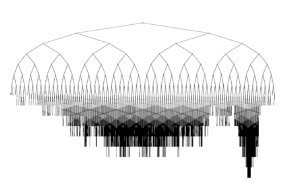
\includegraphics[width=0.49\textwidth,keepaspectratio]{3.png}
			\caption{کاربرد جستجوی درخت مونت کارلو برای الگوریتم ژنتیک}
			\label{fig:fig3}
		\end{figure}
		یک محاسبه سریع برای یک درخت با ضریب انشعاب 10 و عمق 10 نشان می‌دهد که فضای جستجو برابر با 1111111111 است. الگوریتم‌های ژنتیکی معمولاً زمانی که اندازه درخت بزرگ است بهتر عمل می‌کنند و با افزایش اندازه درخت تعداد گره‌های تولید شده به صورت نمایی افزایش می‌یابد و بنابراین فضای جستجو نیز به همین ترتیب افزایش می‌یابد.
		
		\subsection{حفظ یکپارچگی وزن‌ها}
		یک مسئله شناخته شده با الگوریتم‌های ژنتیکی مشکل کنوانسیون‌های رقابتی است که در آن گره‌های فرزند تولید شده به دلیل تکامل قابلیت بقا ندارند و تناسب کمتری دارند. یک مثال در مورد شبکه عصبی یک عملگر تقاطع است که بر روی وزن‌های شبکه عصبی اعمال می‌شود. این عملگر وزن‌ها را جابه‌جا می‌کند و یک جهش تصادفی اعمال می‌کند که می‌تواند بین لایه‌ها و ابعاد گسترش یابد. وزن‌های تغییر یافته ممکن است برای بهینه‌سازی تابع زیان شبکه عصبی داده شده مناسب نباشند و ممکن است منجر به یک راه‌حل نامعتبر شوند.
		
		\subsection{توضیحات داده‌ها}
		داده‌های دیابت برای پیش‌بینی بروز دیابت ملیتوس انتخاب شده‌اند. این ‏مجموعه داده‌ها اصالتاً از موسسه ملی دیابت و بیماری‌های گوارشی و ‏کلیوی می‌باشد. هدف از این مجموعه داده‌ها پیش‌بینی تشخیصی اینکه ‏آیا یک بیمار دیابت دارد یا نه، بر اساس برخی اندازه‌گیری‌های تشخیصی ‏که در مجموعه داده‌ها درج شده است [1]. مجموعه داده‌ها با استفاده از ‏کاهش نمونه‌گیری و شافل تصادفی متعادل شده‌اند. از یک مقیاس‌گذار ‏مین‌مکس برای مقیاس‌گذاری داده‌ها استفاده شده است.‏
		
		\begin{figure}[H]
			\centering
			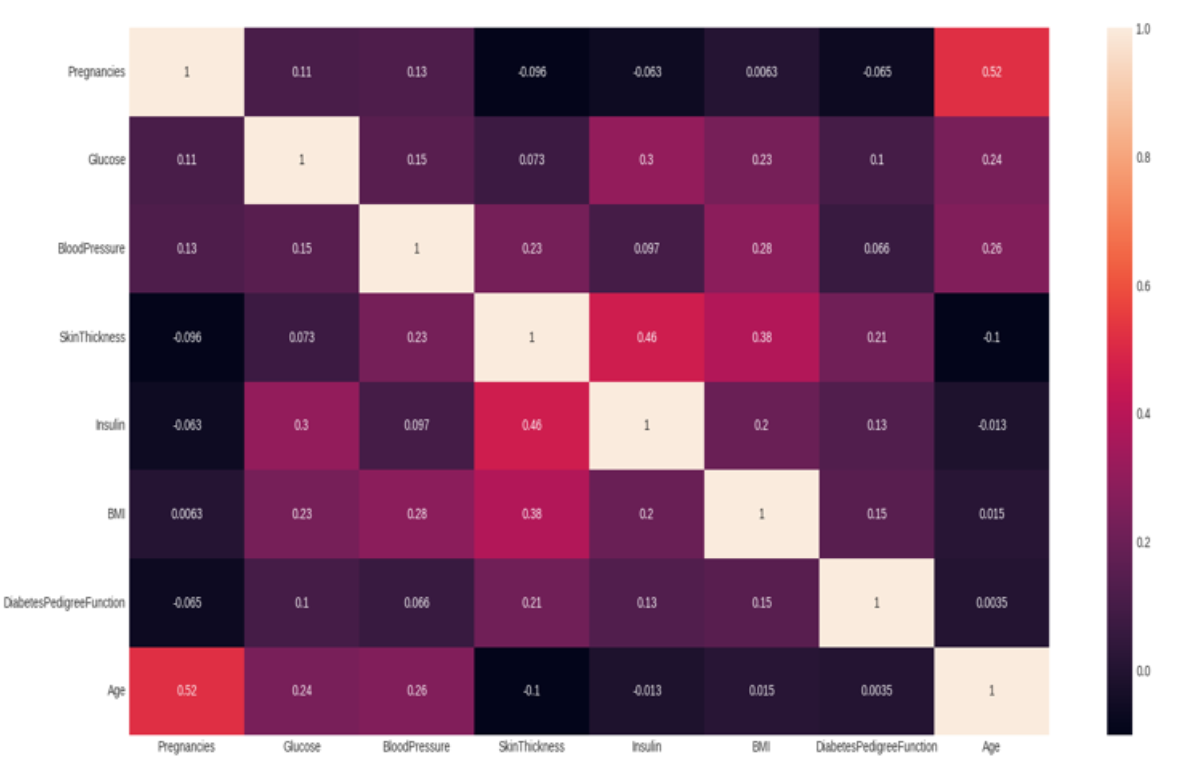
\includegraphics[width=0.49\textwidth,keepaspectratio]{4.png}
			\caption{الگوریتم ژنتیکی ساده}
			\label{fig:fig4}
		\end{figure}
		
		
		این مسئله طبقه‌بندی، ما یک شبکه عصبی پیش‌خور با 4 لایه پنهان ‏توسعه داده‌ایم. این شبکه عصبی دارای 8 گره ورودی و (16-8-4-1) ‏گره پنهان به ترتیب در هر لایه است. شبکه عصبی از تابع فعال‌سازی ‏سیگموید، تابع زیان آنتروپی باینری و بهینه‌ساز آدم با نرخ یادگیری 0.01 ‏استفاده می‌کند. شبکه برای 200 دوره با اندازه دسته 10 آموزش داده شده ‏است.‏
		وزن‌های این شبکه عصبی به عنوان نقطه بهینه‌سازی برای رویکرد ‏MCTS-‎GA‏ ما استفاده می‌شوند. وزن‌های هر لایه برداری شده، ترکیب و ‏برچسب‌گذاری می‌شوند تا یک فرد تشکیل شود که الگوریتم بر روی آن ‏اعمال می‌شود.‏
		\section{رویکرد}
		در رویکرد ما، سعی می‌کنیم به هر دو مسئله ذکر شده با ترکیب ‏رویکردهای ‏MCTS‏ و ‏GA‏ بپردازیم. می‌توانیم از ساختار الگوریتم ‏ژنتیکی بهره‌برداری کنیم زیرا این الگوریتم درختی را تولید می‌کند که ‏مکانیسمی برای ارزیابی پاداش از نظر تناسب فرد دارد. ‏MCTS‏ از همان ‏ساختار درخت زیرین همراه با تابع تناسب برای محاسبه مقدار ‏Q‏ استفاده ‏می‌کند که نشان‌دهنده مجموع تجمعی پاداش‌ها است. مقدار ‏N‏ که ‏نشان‌دهنده تعداد بازدید هر گره است نیز برای محاسبه حدود بالا ‏نگهداری می‌شود. ساختار کلی شامل گسترش کامل گره‌های فرزند با ‏استفاده از ‏GA‏ و استفاده از ‏MCTS‏ با سیاست ‏UCT‏ برای جستجوی ‏گره‌های بهینه با تابع تناسب به عنوان روشی برای اختصاص پاداش‌ها ‏است.‏
		فرایند تکامل با استفاده از ‏GA‏ شامل شروع با یک جمعیت ‏تصادفی است که در مورد ما وزن‌های شبکه عصبی است. جمعیت اولیه ‏P0‎‏ با اندازه مشخص با افزودن یک توزیع یکنواخت تصادفی به هر بُعد از ‏وزن‌های شبکه عصبی و ایجاد فرزندان با وزن‌های تصادفی تولید ‏می‌شود.‏
		در مرحله بعد، مفهوم عمل ژنتیکی برای ‏MCTS‏ را همانطور که با ‏کادر خط‌چین در شکل 5 نشان داده شده است، معرفی می‌کنیم. عمل ‏ژنتیکی شامل سه عمل ژنتیکی زیر است که بر روی جمعیت والدین ‏اعمال می‌شود.‏
		
		•	عمل ژنتیکی ‏
		\\o	انتخاب
		\\o	تقاطع
		\\o	جهش
		
		انتخاب: استراتژی‌های انتخاب مختلفی مانند چرخ رولت، تورنمنت، ‏رتبه‌بندی، حالت ثابت و غیره برای فیلتر کردن افراد با تناسب بیشتر ‏موجود است. مکانیزم انتخاب استفاده شده در این رویکرد انتخاب ‏تورنمنت ‏k‏-راه است. انتخاب تورنمنت انتخاب ‏k‏ فرد تصادفی از جمعیت ‏و انتخاب بهترین تناسب در میان افراد تصادفی انتخاب شده را اعمال ‏می‌کند.‏
		\begin{figure}[H]
			\centering
			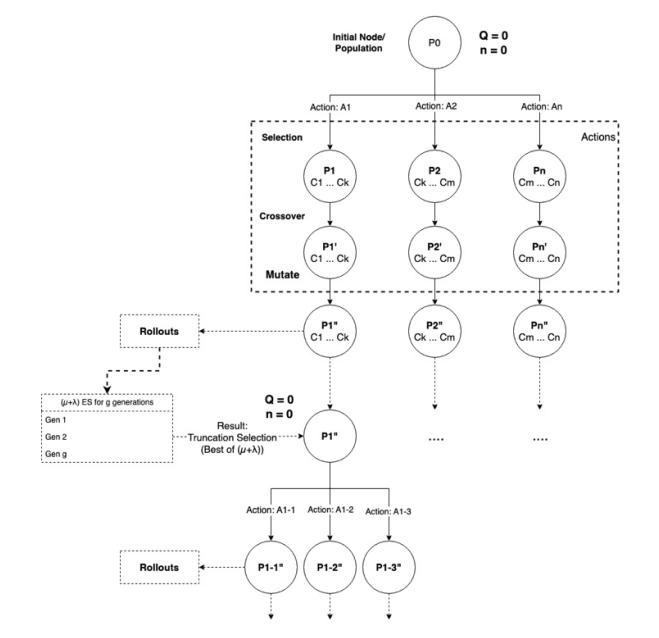
\includegraphics[width=0.49\textwidth,keepaspectratio]{5.png}
			\caption{کاربرد جستجوی درخت مونت کارلو برای الگوریتم ژنتیک}
			\label{fig:fig5}
		\end{figure}
		تقاطع: یک عملگر تقاطع سپس بر روی جمعیت اولیه برای تولید ‏فرزندان اعمال می‌شود. تقاطع یک نقطه‌ای اعمال می‌شود که در آن ‏عملگر تقاطع را به هر لایه از شبکه عصبی محدود کرده‌ایم تا مشکل ‏کنوانسیون‌های رقابتی را کاهش دهیم و یکپارچگی وزن‌های شبکه ‏عصبی را حفظ کنیم.‏
		جهش: عملگر جهش برای معرفی جهش تصادفی در جمعیت ‏استفاده می‌شود. برای رویکرد ما، از جهش تصادفی در هر لایه از شبکه ‏عصبی با جابه‌جایی مقادیر وزن دو فرد به‌طور تصادفی انتخاب شده ‏استفاده کرده‌ایم. گره‌های فرزند بعدی با سیاست ‏UCT‏ از ‏MCTS‏ از ‏گره ریشه تا یافتن یک گره برگ انتخاب می‌شوند. فرزندان در میان ‏گره‌های برگ به‌طور تصادفی انتخاب شده و مقادیر ‏Q‏ و ‏N‏ مربوط به ‏آنها بازگشت داده می‌شود. سیاست ‏UCT‏ با استفاده از ‏UCB1‎‏ به شرح ‏زیر است.‏
		\[ UCT=Q+UCB1 \]
		\[UCB1=\sqrt{\dfrac{c*ln(N)}{N+1}} \]،که در آن ‏Ni‏ گره فرزند ‏i‏-ام و ‏N‏ تعداد گره‌های فرزند است.
		\\معادله حدود بالای اعتماد به نفس
		
		گام بعدی در فرایند اعمال مفهوم رول‌آوت (شبیه‌سازی) بر اساس ‏رویکرد ‏MCTS‏ است. برای گره فرزند انتخاب شده، یک عمل رول‌آوت ‏تکاملی اعمال می‌شود که در آن فرد با استفاده از استراتژی تکاملی (‏‎µ+l‎‏) ‏تکامل می‌یابد، برخلاف شبیه‌سازی‌های عمل تصادفی معمولی که در ‏آزمایشات پژوهشی قبلی انجام شده‌اند [3]. دلیل اعمال رول‌آوت تکاملی ‏این است که ببینیم آیا فرد جهش‌یافته ژنتیکی بیشترین تناسب ممکن را ‏برای فنوتیپ خود دارد یا خیر. ما این فرایند را به عنوان پیر شدن فرد در ‏مقایسه با پدیده زیستی پیر شدن تعریف می‌کنیم. بنابراین، فرایند پیر شدن ‏معرفی شده در رول‌آوت تعیین می‌کند که بهترین سن (نسل) ممکن که ‏در آن فرد بهترین تناسب را برای جهش ژنتیکی مجدد دارد کدام است. ‏فرایند رول‌آوت/پیر شدن فرد را جایگزین خواهد کرد اگر تناسب بهتری در ‏نسل‌های بعدی استراتژی تکاملی یافت شود.‏
		این فرایند تا رسیدن به عمق مشخص شده درخت تکرار می‌شود. ‏این رویکرد انعطاف‌پذیری محاسباتی را از نظر پارامترهای قابل تنظیم ‏مانند ارتفاع درخت، انتخاب تورنمنت، تعداد نسل‌های رول‌آوت و ضریب ‏انشعاب فراهم می‌کند. این پارامترها می‌توانند به صورت ترکیبی با یکدیگر ‏بر اساس ظرفیت محاسباتی موجود استفاده شوند. بنابراین، کاربرد عمل ‏ژنتیکی و رول‌آوت تکاملی در ترکیب با ‏MCTS‏ اساس رویکرد مورد ‏بحث در این مقاله را فراهم می‌کند
		
		\section{نتایج}
		رویکرد ‏MCTS-GA‏ یک مکانیزم نوین برای بهینه‌سازی است و هدف آن ‏بی‌تفاوت بودن نسبت به داده‌ها است. نمایش الگوریتم ژنتیکی می‌تواند به ‏روش‌های مختلفی پیکربندی شود که این رویکرد را برای طیف گسترده‌ای ‏از مسائل بهینه‌سازی مناسب می‌سازد. در این آزمایش، ‏MCTS-GA‏ با ‏استفاده از ‏UCT‏ برای ۲۰ نسل (عمق درخت) با شبیه‌سازی‌هایی که برای ‏‏۱۰ نسل و ضریب انشعاب ۵ تنظیم شده بودند، اجرا شد. ‏GA‏ برای ۲۰۰ ‏نسل اجرا شد و شبکه عصبی برای ۲۰۰ ایپاک اجرا شد.‏
		نتایج به‌دست‌آمده از آزمون اولیه مثبت بود. رویکرد ‏MCTS-GA‏ توانست ‏وزن‌های شبکه عصبی را برای طبقه‌بندی بهتر داده‌های دیابت ‏بهینه‌سازی کند و نتایج دقت بهتری به دست آورد.‏
		مقایسه نتایج به‌دست‌آمده با نتایج شبکه عصبی اصلی و الگوریتم ژنتیک کانونی ‏در جدول زیر نشان داده شده است.‏
		\begin{figure}[H]
			\centering
			\caption{نتایج دقت}
			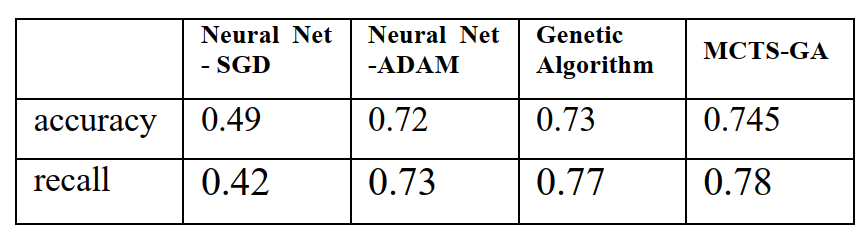
\includegraphics[width=0.49\textwidth,keepaspectratio]{6.png}
			\label{fig:fig6}
		\end{figure}
		دقت طبقه‌بندی نیز از منحنی‌های ‏roc-auc‏ نشان داده شده در زیر قابل ‏مشاهده است.‏
		\begin{figure}[H]
			\centering
			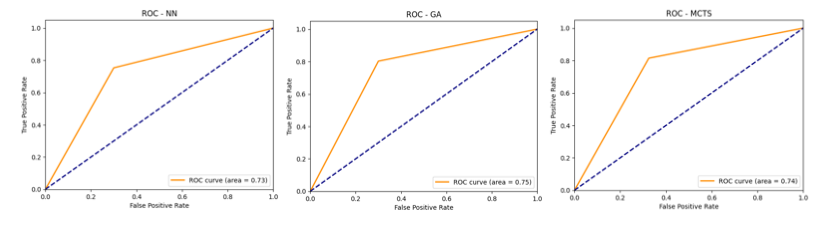
\includegraphics[width=0.49\textwidth,keepaspectratio]{7.png}
			\caption{منحنی ‏ROC-AUC‏ برای شبکه عصبی، الگوریتم ژنتیک و ‏MCTS-GA‏ به ترتیب‏}
			\label{fig:fig7}
		\end{figure}
		ماتریس ابهام برای سه رویکرد مقایسه شده در زیر نشان داده شده است.‏
		\begin{figure}[H]
			\centering
			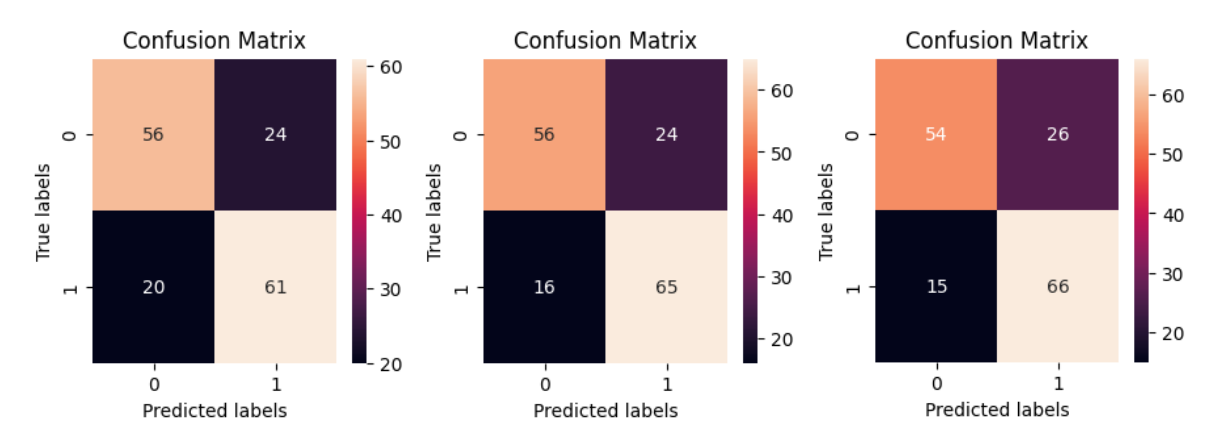
\includegraphics[width=0.49\textwidth,keepaspectratio]{8.png}
			\caption{ماتریس ابهام برای شبکه عصبی، الگوریتم ژنتیک و ‏MCTS-‎GA‏ به ترتیب.‏}
			\label{fig:fig8}
		\end{figure}
		
		\section{بحث}
		آزمایش تأیید می‌کند که‎ MCTS-GA ‎در بهینه‌سازی وزن‌های شبکه ‏عصبی کار می‌کند. بهینه‌سازی وزن‌ها و در نتیجه طبقه‌بندی بهتر توسط‎ ‎MCTS-GA ‎نسبت به الگوریتم ژنتیک و رویکرد شبکه عصبی ‏پیش‌خورشی دیده می‌شود. اگرچه بهبود زیاد نیست، اما‎ MCTS-GA ‎در مقایسه با دو تکنیک دیگر در زمان قابل مقایسه اجرا می‌شود. برای ‏بهبود الگوریتم مورد بحث در اینجا و آزمایش نمایش‌های مختلف مسائل، ‏فضای بهبود وجود دارد. به‌طور کلی، ما یک رویکرد نوین را بحث کردیم ‏که می‌تواند به‌عنوان یک تکنیک قوی و معتبر برای تکنیک‌های ‏بهینه‌سازی در آینده اثبات شود.‏
    \renewcommand{\refname}{مراجع}
		\begin{LTR}
			\begin{thebibliography}{99} 
				
				\bibitem{Smith88} Smith JW, Everhart JE, Dickson WC, Knowler WC, Johannes RS. Using the ADAP Learning Algorithm to Forecast the Onset of Diabetes Mellitus. Proc Annu Symp Comput Appl Med Care. 1988 Nov 9:261–5.
				\bibitem{Goldberg13} Goldberg, David E. Genetic algorithms. Pearson Education India, 2013.
				\bibitem{Silver17} Silver, D., Schrittwieser, J., Simonyan, K. et al. Mastering the game of Go without human knowledge. Nature 550, 354–359 (2017).
				
				\bibitem{Lee95} K. W. Lee and H. N. Lam, "Optimising neural network weights using genetic algorithms: a case study," Proceedings of ICNN'95 – International Conference on Neural Networks, Perth, WA, Australia, 1995, pp. 1384-1388 vol.3.
				
				\bibitem{Sheta12} Sheta, Alaa, Braik, Malik, Aljahdali, Sultan. (2012). Genetic Algorithms: A tool for image segmentation. Proceedings of 2012 International Conference on Multimedia Computing and Systems, ICMCS 2012. 84-90. 10.1109/ICMCS.2012.6320144.
				
				\bibitem{LoBosco01} G. Lo Bosco, "A genetic algorithm for image segmentation," Proceedings 11th International Conference on Image Analysis and Processing, Palermo, Italy, 2001, pp. 262-266.
				
				\bibitem{Rocki11} K. Rocki and R. Suda, "Large-Scale Parallel Monte Carlo Tree Search on GPU," 2011 IEEE International Symposium on Parallel and Distributed Processing Workshops and Phd Forum, Anchorage, AK, USA, 2011, pp. 2034-2037, doi: 10.1109/IPDPS.2011.370.
				
				\bibitem{Lambora19} Lambora, K. Gupta and K. Chopra, "Genetic Algorithm- A Literature Review," 2019 International Conference on Machine Learning, Big Data, Cloud and Parallel Computing (COMITCon), Faridabad, India, 2019, pp. 380-384, doi: 10.1109/COMITCon.2019.8862255.
				
				\bibitem{Kuo20} Jonathan C.T. Kuo, "Genetic Algorithm in Artificial Neural Network and its Optimization Methods","medium.com", Web, 2020.
				
				\bibitem{Sharma18}SagarSharma,"MCTS",
				"https://towardsdatascience.com/", Web, 2018.
				
			\end{thebibliography}
		\end{LTR}
	\end{multicols}
\end{document}